\documentclass[11pt]{article}
\usepackage[a4paper, margin=20mm]{geometry}
\usepackage{hyperref}

\usepackage{amsmath}
\usepackage{physics}

\usepackage{graphicx}
\graphicspath{ {./figs/} }
\usepackage{subfig}

%\renewcommand{\baselinestretch}{2}
\usepackage{setspace}
\doublespacing
\usepackage{titlesec}
\usepackage{authblk}
\usepackage{titling}
\usepackage[backend=biber,
style=authoryear,
citestyle=apa]{biblatex}
\addbibresource{Reference.bib} % The filename of the bibliography

\usepackage{enumitem}

\titlespacing\section{0pt}{0pt plus 0pt minus 0pt}{0pt plus 2pt minus 2pt}
\titlespacing\subsection{0pt}{0pt plus 4pt minus 2pt}{0pt plus 2pt minus 2pt}
\titlespacing\subsubsection{0pt}{0pt plus 4pt minus 2pt}{0pt plus 2pt minus 2pt}

\usepackage{amsfonts}

\begin{document}

\begin{titlepage} % Suppresses displaying the page number on the title page and the subsequent page counts as page 1
	\newcommand{\HRule}{\rule{\linewidth}{0.5mm}} % Defines a new command for horizontal lines, change thickness here
	
	\center % Centre everything on the page
	
	%------------------------------------------------
	%	Headings
	%------------------------------------------------
	
	\textsc{\LARGE University of Oxford}\\[1.5cm] % Main heading such as the name of your university/college
	
	\textsc{\Large Engineering Science}\\[0.5cm] % Major heading such as course name
	
	\textsc{\large 4YP Report}\\[0.5cm] % Minor heading such as course title
	
	%------------------------------------------------
	%	Title
	%------------------------------------------------
	
	\HRule\\[0.4cm]
	
	{\huge\bfseries The Future of Work}\\[0.4cm] % Title of your document
	
	\HRule\\[1.5cm]
	
	%------------------------------------------------
	%	Author(s)
	%------------------------------------------------
	
	\begin{minipage}{0.4\textwidth}
		\begin{flushleft}
			\large
			\textit{Author}\\
			Terence \textsc{Tan} % Your name
		\end{flushleft}
	\end{minipage}
	~
	\begin{minipage}{0.4\textwidth}
		\begin{flushright}
			\large
			\textit{Supervisor}\\
			Professor Michael A \textsc{Osborne} % Supervisor's name
		\end{flushright}
	\end{minipage}
	
	% If you don't want a supervisor, uncomment the two lines below and comment the code above
	%{\large\textit{Author}}\\
	%John \textsc{Smith} % Your name
	
	%------------------------------------------------
	%	Date
	%------------------------------------------------
	
	\vfill\vfill\vfill % Position the date 3/4 down the remaining page
	
	{\large\today} % Date, change the \today to a set date if you want to be precise
	
	%------------------------------------------------
	%	Logo
	%------------------------------------------------
	
	\vfill\vfill
	
\includegraphics[width=0.5\textwidth]{/Users/terencetan/Documents/Uni stuff/Engineering Science/4YP/4YP-The-Future-of-Work/Report/Figures/logo.png}\\[1cm] % Include a department/university logo - this will require the graphicx package
	 
	%----------------------------------------------------------------------------------------
	
	\vfill % Push the date up 1/4 of the remaining page
	
\end{titlepage}

\begin{abstract}
	I would like to express my deepest gratitude to Professor Michael Osborne for supervising me throughout this project. His insights and guidance are very much appreciated. This project would not have been possible without the dataset provided by him.
   \end{abstract}

\section*{Acknowledgements}

	\thispagestyle{empty}
   I would like to express my deepest gratitude to Professor Michael Osborne for supervising me throughout this project. His insights and guidance are very much appreciated. This project would not have been possible without the dataset provided by him.


\newpage


\section{Introduction}
\label{sec:Introduction}

Technological advancement is widely believed to be the primary driving force behind economic growth (\cite{RePEc:ssa:lembks:dosietal-1988}). At the same time, there is potential for technological displacement of labour. This concept of 'technological unemployment' was first introduced by David Ricardo in the 19th century (\cite{WoirolGregoryR1997Ttua}), who wrote that he had become "convinced that the substitution of machinery for human labour, is often very injurious to the interests of the class of labourers" (\cite{10.1257/jep.33.2.229}). This idea was further explored by John Maynard Keynes, who blamed "our discovery of means of economising the use of labour outrunning the pace at which we can find new uses for labour" for potential widespread technological unemployment (\cite{Keynes2010}). However, there are those that are cautiously optimistic of the impact of technological advances on labour. Prominent member of the United Automobile Workers union Walter Reuther and his colleague had hopes that automation could eliminate the drudgery of industrial work and ultimately allow workers to pursue leisurely interests. Yet, even they shared fears that automation could lead to widespread structural unemployment if not managed properly (\cite{SteigerwaldDavid2010WRtU}). Alas, history seems to have validated their fears; the proportion of manufacturing employment in the US among non-agricultural workers decreased from 32\% in 1955 to 8\% in 2019 (\cite{rose_2021}). That being said, there is no consensus on the impact of technological advances on the decline of the manufacturing sector relative to other factors such as globalisation and offshoring (\cite{RoseElizabethL.2021TDoU}) (\cite{krugman2019globalization}).

At the same time, ageing population is a social issue that has become increasingly relevant all over the world (\cite{2002Wpa1}).

\subsection{Ageing Population}
\label{subsec:ageingpopulation}

The world population is ageing over the next few decades (\cite{science}). The rising elderly to working age population ratio is increasing and will continue to do so (\cite{WHO}). This trend is known as an ageing population, and will strain the public and social services of many countries around the world (\cite{publicservicesstrain}). As one of the key social challenges facing the world for the next few decades, it would be interesting to examine how an ageing population will affect the economy, and in particular, the job market and the interplay with automation in the workplace. As more workers age out of the workforce, automation is expected to make up for it (\cite{futureofemployment}).

\subsection*{Related Works}
Research into the social implications of an ageing population had been carried out as far back as 2002. \cite{tinker2002social} outlined the demographic trends around the turn of the millennium that pointed to the future of an ageing world, and highlighted the falling potential support ratio (ratio of people aged 15-64 to people aged 65 and above) around the world, which will affect the distribution of resources, such as in the case of pensions, of a country. This study also talked about the relative power between the young and old, and pointed out that the older generation will have larger share of votes, potentially wielding more political power. Indeed, contemporary authors, such as \cite{Munger+2022}, have noted this power struggle between the older and younger generations. The US government has also been described as a gerontocracy (\cite{noah_2019}) (\cite{thompson_2020}) in modern times. The numbers back this up, with the average age of a US senator being 64 in 2021 (\cite{manning_2022}).

\cite{Cheng2020} conducted a global analysis of population ageing and mortality between 1990 and 2017, and concluded that there was a pattern of higher disease-related deaths due to population ageing around the world within that time period. The study recommended policies aimed at encouraging healthy ageing.

\subsection*{Cross-country comparison}
\label{subsec:crosscountrycomparison}
In the US, there is evidence to suggest that the country's healthcare system is not prepared to meed the increasing demands of the ageing population (\cite{foley_retooling_2020}).

While this paper will be focusing on the US, there are numerous other studies looking into ageing population of the US as well as other countries and regions of the world. China is expected to age rapidly over the next few decades (\cite{BeardsonTimothy2021Ag:C}), and studies such as \cite{LuoYanan2021TaCf} examined this phenomenon in the context of the country.

\subsection{Project Overview}
\label{subsec:projectoverview}
In this project, we aim to examine the relationship between the age distribution within occupations and the degree of automation (\cite{futureofemployment}) of those occupations. Although similar work has been done on this topic (\cite{twinthreats}), the study only looked at broad categories of employment. In this project, we will zoom in to look at specific occupations. We might also look into any correlations with the skills/knowledge required for those occupations. This will all be done using the scikit-learn library\footnote{https://scikit-learn.org/stable/} in Python. Specifically, we will look at a Bayesian non-parametric machine learning technique known as Gaussian Process (\cite{GaussianProcess}); this model was used in previous work (\cite{futureofemployment}), and so, would be a good model to start with. We will test and validate against different models and pick the best performing ones.

We will be using the proportion of elderly people as a metric for measuring the `age' of occupations. We acknowledge that the definition of elderly age varies across different countries and cultures (\cite{ageingculture}), and that the ageing process varies for different people depending on a variety of factors (\cite{levine2013modeling})(\cite{hayflick2007biological}). In fact, there are studies looking into moving beyond using chronological age to define an elderly person (\cite{KotterGrhn2015})(\cite{SOTOPEREZDECELIS2018e305})(\cite{klemera2006new}). However, there are numerous issues surrounding this approach (\cite{jylhava2017biological}), such as validation of such results are often difficult (\cite{biologicalagedifficult}), resulting in little consensus on an alternative metric to chronological age. For this reason, we will stick to the conventional definition of 65 years and older as `elderly' (\cite{who2010definition})(\cite{orimo2006reviewing})(\cite{oecddata}). This definition is also convenient for us since the oldest age group featured in our datasets are 65 years and older. Hence, it would make sense to have the metric for measuring the `age' of an occupation be the ratio of people aged 65 years and older to the total number of people in that particular occupation. We will refer to this metric as the Elderly Proportion (EP). However, we also recognise that this definition of 'elderly' coincides with the retirement age of the US (\cite{MunnellAliciaH2013SSRR}). Hence, using this metric alone might lead to misleading results since we would expect people in that age group to leave the workforce. It might be better to use the proportion of 55 years and older as a metric, i.e. the ratio of people aged 55 years and older to the total number of people, since this figure might be more robust to the effects of retirement on labour force participation. We shall refer to this metric as the Old Proportion (OP). Having said that, the Elderly Proportion would still prove to be an interesting metric to investigate. For example, if there is a general trend of increasing EP over the years, that would be a sign of an ageing labour force in spite of the effects of retirement. Therefore, we shall examine both of these metric in this paper.

\subsection*{Related Works}

\newpage

\section{Dataset}
\label{sec:Dataset}
We used two main metrics for this project: the automatability of occupations, and the age distribution within occupations. The dataset for the former is provided in an earlier work by \cite{futureofemployment}. The latter can be found in datasets provided by the US Bureau of Labour Statistics\footnote{https://www.bls.gov} (BLS); there is one dataset for each year from 2011 to 2021. All the datasets mentioned above use the Standard Occupational Classification (SOC) to classify the occupations, which means that we can map from one dataset to the another using the SOC codes\footnote{https://www.bls.gov/soc/2018/soc\_structure\_2018.pdf}. However, it is necessary to perform some data wrangling before we can proceed with the mapping. Additionally, changes were made to the SOC in 2018, so we would have to standardise all the datasets. In the following sections, we shall examine the datasets and the required data wrangling in more detail.

\subsection{BLS Dataset}
\label{subsec: BLS}
As mentioned in Chapter \ref{sec:Dataset}, the BLS provides one dataset for each year from 2011 to 2021. The datasets from 2011 to 2019 follow the old SOC while the 2020 and 2021 ones follow the updated version. We want to standardise everything according to the updated SOC. We first label each dataset with the respective year and concatenate  all of them along the row axis; we shall refer to this concatenated dataset as the BLS dataset for the rest of the paper. A section of the BLS dataset can be seen in Figure \ref{fig:df}. Note that the numbers under the \emph{Total} and age group columns are in thousands. Furthermore, the median age is not provided for all occupations, which makes it less useful as a metric. Hence, we will not be using it in this paper.

\begin{figure}[!htb]
    \centering
    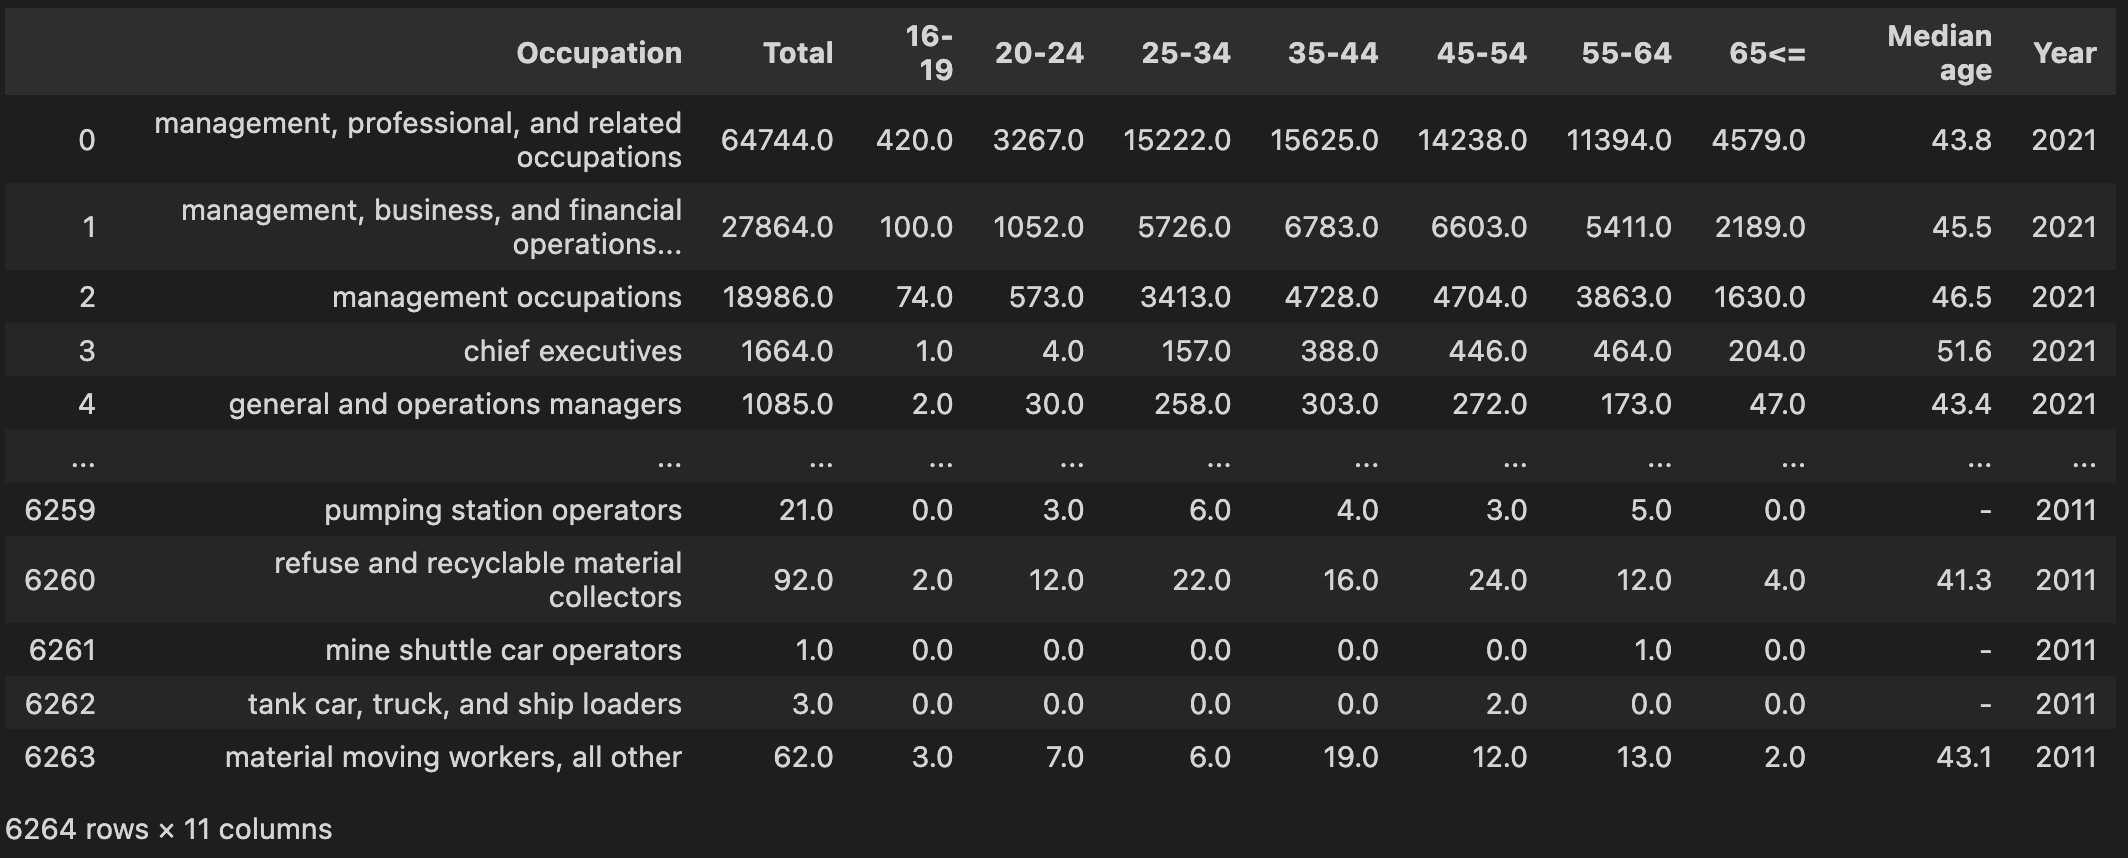
\includegraphics[width=12cm]{/Users/terencetan/Documents/Uni stuff/Engineering Science/4YP/4YP-The-Future-of-Work/Report/Figures/BLS dataset (before).png}
    \caption{BLS dataset (before processing)}
	\label{fig:df}
\end{figure}

While the BLS did provide documents\footnote{https://www.bls.gov/soc/2018/home.htm} outlining and explaining the changes to the SOC, it is generally too vague to be anything more than a rough guide. Furthermore, some of the changes made to the SOC are fairly complex. In addition to that, the BLS collected data differently for some occupations after 2019. For example, both `Marketing Managers' (SOC code: 11-2021) and `Sales Managers' (SOC code: 11-2022) are classified under `Marketing and Sales Managers' (SOC code: 11-2020). From 2011 to 2019, the BLS only collected data for `Marketing and Sales Managers' while they collected data for `Marketing Managers' and `Sales Managers' separately in 2020 and 2021. While this represents more detailed data, it is inconsistent with data collected in previous years.

In order to list out all the changes and inconsistencies, we use the \emph{pandas.DataFrame.join} function to join an old SOC dataset (from 2011 to 2019) with an updated SOC dataset (from 2020 to 2021) using the \emph{Occupation} column. We can then obtain a list of occupations from the old SOC dataset which did not join, and a corresponding list for the updated SOC dataset. We then manually go through both lists and decide on how to standardise the BLS dataset. While this process is tedious, it is reasonably doable since each list only contains about a hundred rows. The changes and rationale for them are listed alongside the occupations in both lists. All of these are placed in an Excel file\footnote{https://github.com/terencetan-c/4YP-The-Future-of-Work/blob/main/Data\%20cleaning/Changes.xlsx}.

The list of actions required are as follows: -, Delete, Change, Combine, Combine but keep. The dash indicates that no action is required. `Delete' means to delete the occupation; this is usually because the particular occupation no longer exists under the new SOC. `Change' indicates a name change. `Combine' indicates that two or more occupations should be combined into the overarching occupation. For example, the two occupations mentioned before, `Marketing Managers' and `Sales Managers', will be combined into `Marketing and Sales Managers' to ensure consistency in the BLS dataset across the years. This will basically be an element-wise addition of the rows, involving only the \emph{Total} and age group columns. This is another reason why we dropped the \emph{Median age} column since we have no way of combining median values for the BLS dataset. Lastly, the `Combine but keep' action is used in cases where we have to combine to maintain consistency but are still able to preserve some granularity by keeping the original rows. For example, the old SOC classifies the four occupations `Home Health Aides' (31-1011), `Psychiatric Aides' (31-1013), `Nursing Assistants' (31-1014), and `Orderlies' (31-1015) under `Nursing, Psychiatric, and Home Health Aides' (31-1000 and 31-1010). Additionally, the old SOC also has `Personal Care Aides' (39-9020 and 39-9021) classified separately. The new SOC renamed `Nursing, Psychiatric, and Home Health Aides' to `Home Health and Personal Care Aides; and Nursing Assistants, Orderlies, and Psychiatric Aides' (and changed the SOC code from 31-1000 to 31-1100) and moved `Personal Care Aides' (now 31-1122) under this newly named occupation. Another thing to note is that the datasets following the old SOC only collected data of `Nursing, Psychiatric, and Home Health Aides' as a whole instead of the four occupations individually. They also collected data for `Personal Care Aides'. On the other hand, the datasets following the new SOC collected data for the four occupations, `Home Health Aides' (now 31-1121), `Psychiatric Aides' (now 31-1133), `Nursing Assistants' (now 31-1131), and `Orderlies' (now 31-1132), and the newly moved occupation, `Personal Care Aides', separately. Note that both groups of datasets have data of `Personal Care Aides' on its own, and we would like to keep it that way to preserve granularity of the data. For the datasets following the old SOC, we would apply `Combine' on `Nursing, Psychiatric, and Home Health Aides' (effectively just a name change in this case) and `Combine but keep' on `Personal Care Aides'. For the new SOC datasets, we apply `Combine' on the four occupations and `Combine but keep' on `Personal Care Aides'. This way, we end up with data for a combined `Nursing, Psychiatric, and Home Health Aides' to `Home Health and Personal Care Aides; and Nursing Assistants, Orderlies, and Psychiatric Aides', while simultaneously still retaining `Personal Care Aides'.

Having systematically gone through all the inconsistencies and indicating one of the five actions required for the inconsistencies, we then use Python to automate the standardisation process. This gives us the standardised BLS dataset.

One more thing to note is that the occupations in the BLS dataset are not labelled with their respective SOC codes. This is easily rectified once the above data wrangling is completed by joining (on \emph{Occupation}) the BLS dataset with the list of SOC codes to map from occupation name to code.

\subsection{Automatability Dataset}

This dataset (which we shall refer to as Automatability dataset) was obtained from \cite{futureofemployment}, and features 702 Detailed Occupations. For each of these occupations, a Probability of Computerisation\footnote{Defined as 'job automation by means of computer-controlled equipment' by \cite{osborne2017future}} had been calculated. We shall refer to this probability as PCom. Other variables are included as well, such as the skills associated with each occupation and a Category Label. These were used to calculate the PCom, but we will just focus on the PCom in this paper.

\newpage

\section{Preliminary Findings}
\label{sec:prelim findings}

In order to make sense of how well the BLS dataset represents the US labour force, we plot the ratio of the total labour numbers provided by the BLS dataset for each year to the total US civilian labour force\footnote{https://www.bls.gov/cps/cpsaat01.htm} for that year. We do that for \emph{Major Group}, \emph{Minor Group}, \emph{Broad Group}, and \emph{Detailed Occupation} separately. The resulting plots can be seen in Figure \ref{proportion}. Clearly, \emph{Major Group} occupations are most representative of the US civilian labour force, with \emph{Minor Group} being the least. Looking through the BLS dataset, this makes sense since the BLS tended to mostly collect high-level data (\emph{Major Group}) and low-level data (\emph{Broad Group} and \emph{Detailed Occupation}). Another thing to note is that many \emph{Broad Group} occupations only contain a single \emph{Detailed Occupation} which also shares the same occupation name (for example, \emph{Chief Executives}: 11-1010 and 11-1011). Hence, it is not surprising that the ratios for \emph{Broad Group} and \emph{Detailed Occupation} are so similar.

It is important to consider the fact that the US civilian labour force includes both the employed and the unemployed. In years with unusual levels of unemployment rate, the ratios will be distorted and paint a misleading picture. Indeed, we see in Figure \ref{proportion} that there is a considerable dip in the ratios in 2020 relative to other years, coinciding with the onset of the COVID-19 pandemic (\cite{covid2020unemployment})(\cite{congresscovidunemployment}). Plotting the ratios relative to the employed portion of the US civilian labour force accounts for this; as seen in Figure \ref{proportionemp}, the dip in 2020 is no longer present. We can also see that the unemployment rate did not distort the ratios significantly. Hence, our conclusion from before still holds: the \emph{Major Group} is most representative of the US civilian labour force. With that in mind, we will try to use \emph{Major Group} data as much as possible and exercise caution when using \emph{Detailed Occupation} and \emph{Broad Group} data. As for \emph{Minor Group} data, we will neglect it given its low representation of the labour force.



\begin{figure}[!htb]
	\centering
	\subfloat[Major Group]{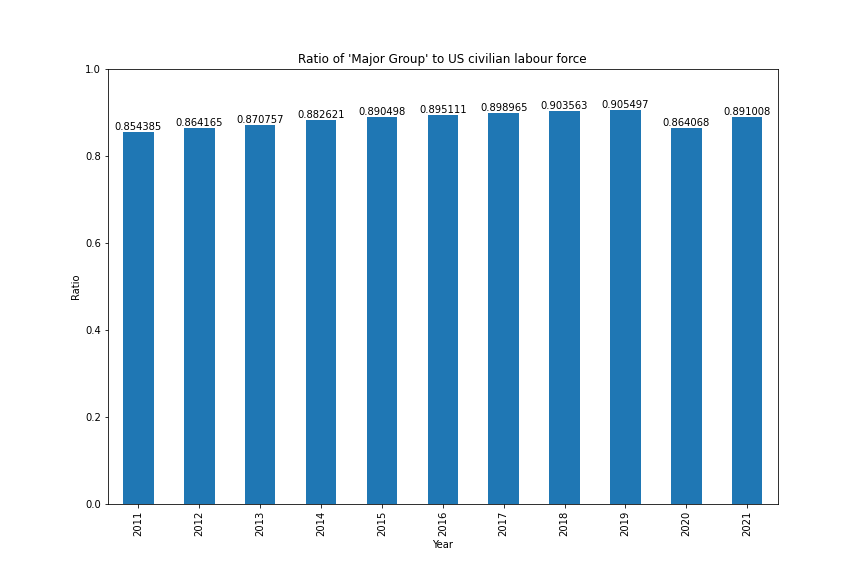
\includegraphics[width=8.5cm]{/Users/terencetan/Documents/Uni stuff/Engineering Science/4YP/4YP-The-Future-of-Work/Report/Figures/Proportion Major.png}\label{fig:promajor}}
	  \hfill
	\subfloat[Minor Group]{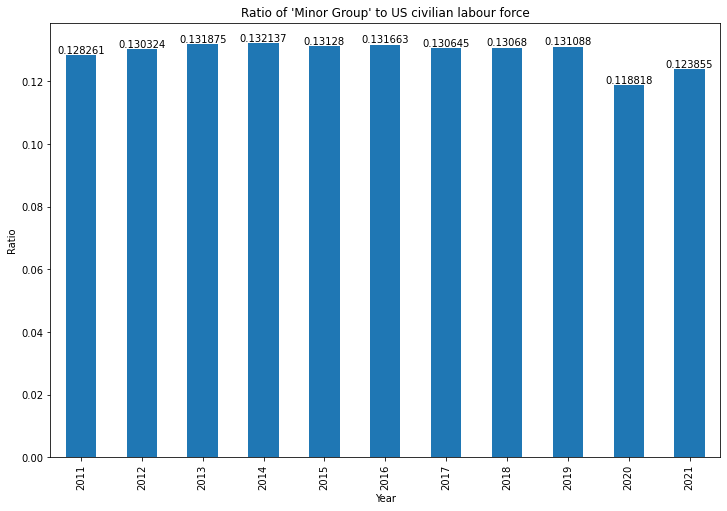
\includegraphics[width=8.5cm]{/Users/terencetan/Documents/Uni stuff/Engineering Science/4YP/4YP-The-Future-of-Work/Report/Figures/Proportion Minor.png}\label{fig:prominor}}
	\hfill
	\subfloat[Broad Group]{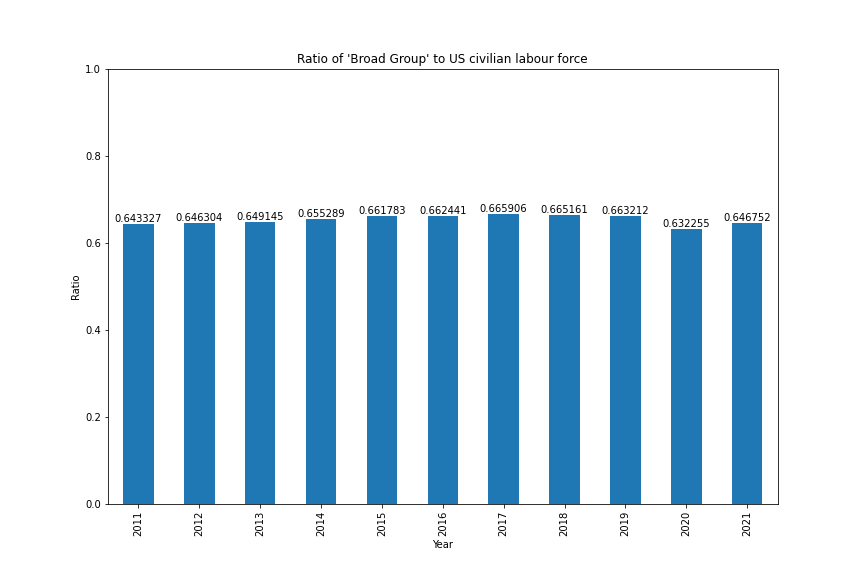
\includegraphics[width=8.5cm]{/Users/terencetan/Documents/Uni stuff/Engineering Science/4YP/4YP-The-Future-of-Work/Report/Figures/Proportion Broad.png}\label{fig:probroad}}
	\hfill
	\subfloat[Detailed Occupation]{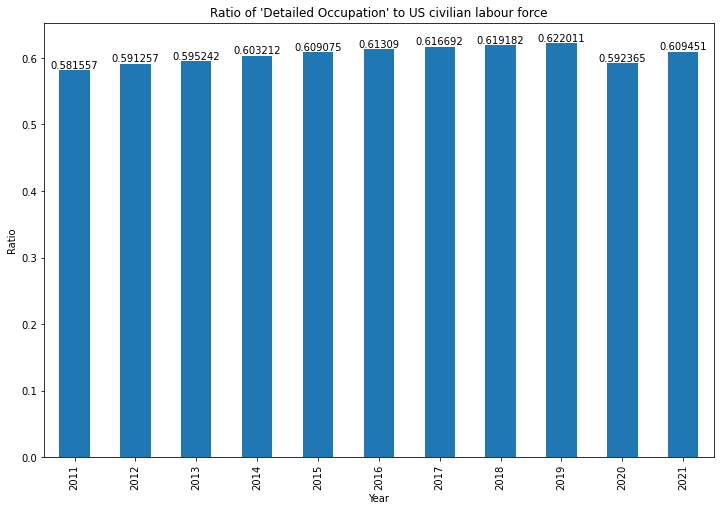
\includegraphics[width=8.5cm]{/Users/terencetan/Documents/Uni stuff/Engineering Science/4YP/4YP-The-Future-of-Work/Report/Figures/Proportion Detailed.png}\label{fig:prodetailed}}
	\hfill
	\caption{Ratio of the various SOC categories to the US civilian labour force}
	\label{proportion}
  \end{figure}
  
\begin{figure}[!htb]
	\centering
	\subfloat[Major Group]{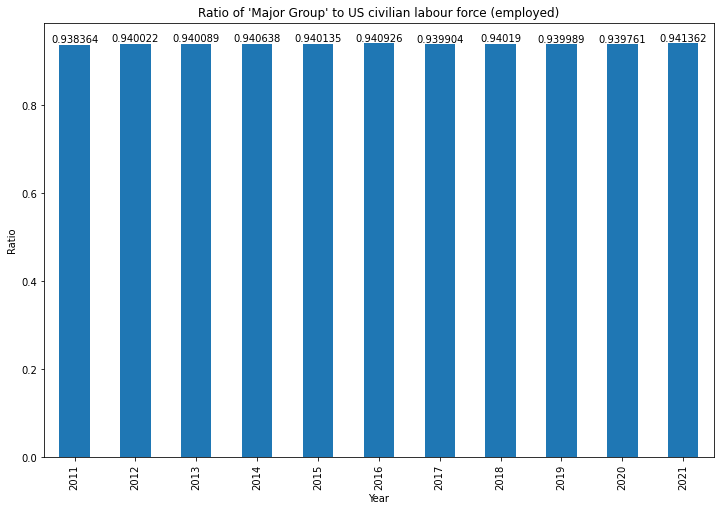
\includegraphics[width=8.5cm]{/Users/terencetan/Documents/Uni stuff/Engineering Science/4YP/4YP-The-Future-of-Work/Report/Figures/Proportion Major (employed).png}\label{fig:empmajor}}
	\hfill
	\subfloat[Minor Group]{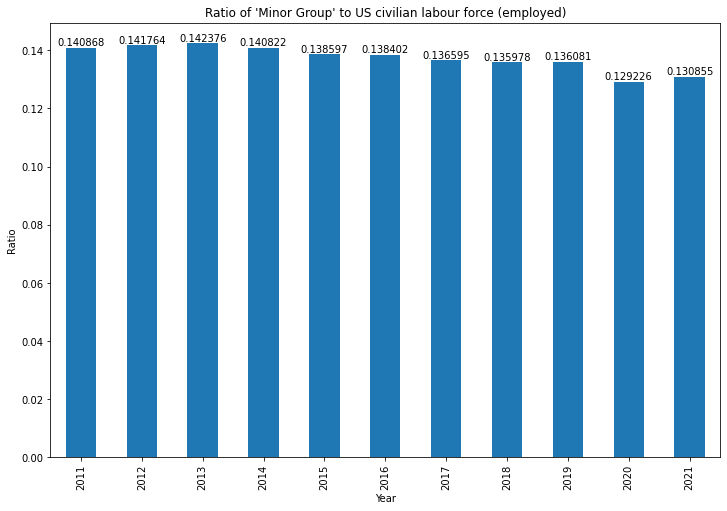
\includegraphics[width=8.5cm]{/Users/terencetan/Documents/Uni stuff/Engineering Science/4YP/4YP-The-Future-of-Work/Report/Figures/Proportion Minor (employed).png}\label{fig:empminor}}
	\hfill
	\subfloat[Broad Group]{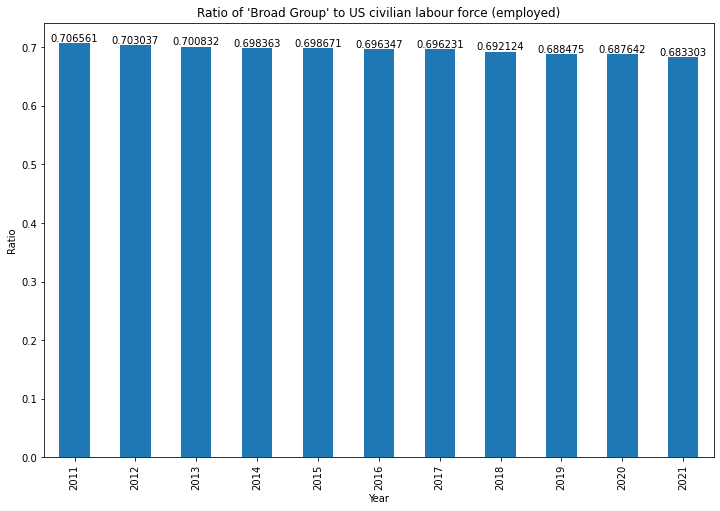
\includegraphics[width=8.5cm]{/Users/terencetan/Documents/Uni stuff/Engineering Science/4YP/4YP-The-Future-of-Work/Report/Figures/Proportion Broad (employed).png}\label{fig:empbroad}}
	\hfill
	\subfloat[Detailed Occupation]{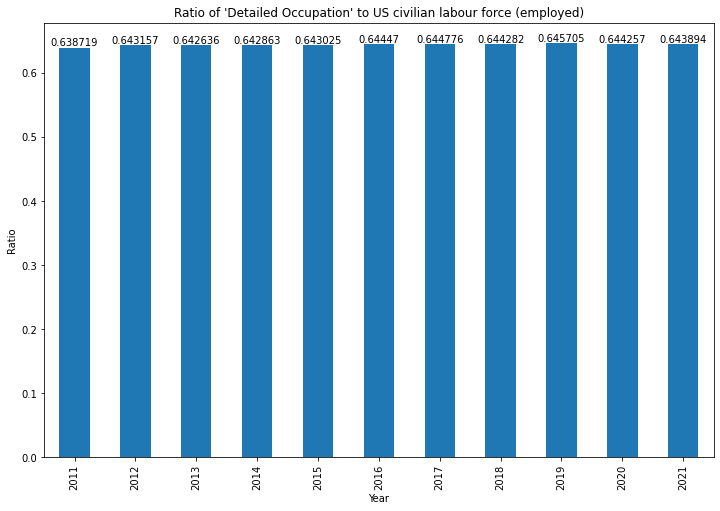
\includegraphics[width=8.5cm]{/Users/terencetan/Documents/Uni stuff/Engineering Science/4YP/4YP-The-Future-of-Work/Report/Figures/Proportion Detailed (employed).png}\label{fig:empdetailed}}
	\hfill
	\caption{Ratio of the various SOC categories to the US civilian labour force (employed)}
	\label{proportionemp}
\end{figure}
    
\subsection{General Trends}
\label{subsec:generaltrends}
We average the EP (refer to Chapter \ref{subsec:projectoverview} for definition) over the Major Groups for each year, and plot the values against the years to obtain Figure \ref{fig:averageEP}. We do the same for OP, and get the plot in Figure \ref{fig:averageOP}. We see a steady increase over the years for both plots, which is not surprising given the ageing population of the US as discussed in Chapter \ref{subsec:crosscountrycomparison}. We can examine these plots in further detail by plotting the EP/OP for each of the 21 Major Groups against the years to obtain Figure \ref{fig:EP/OP against year}; we can see that there is generally an increase across the Major Groups. We do not break down the plots into further detail (for example looking at individual Detailed Occupations) since that will result in plots that are too messy to give us any useful insights.



\begin{figure}[!htb]
	\centering
	\subfloat[Elderly Proportion]{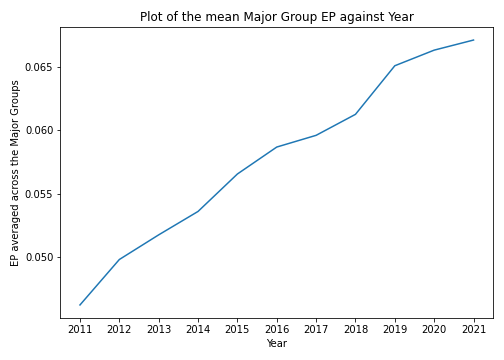
\includegraphics[width=8cm]{/Users/terencetan/Documents/Uni stuff/Engineering Science/4YP/4YP-The-Future-of-Work/Report/Figures/Mean Major Group Elderly Proportion against Year.png}\label{fig:averageEP}}
	\hfill
	\subfloat[Old Proportion]{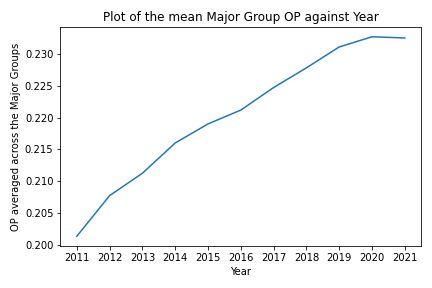
\includegraphics[width=8cm]{/Users/terencetan/Documents/Uni stuff/Engineering Science/4YP/4YP-The-Future-of-Work/Report/Figures/Mean Major Group Old Proportion against Year}\label{fig:averageOP}}
	\hfill
	\caption{Plot of EP/OP (averaged over the Major Groups) against Year}
\end{figure}


\begin{figure}[!htb]
	\centering
	\subfloat[Elderly Proportion]{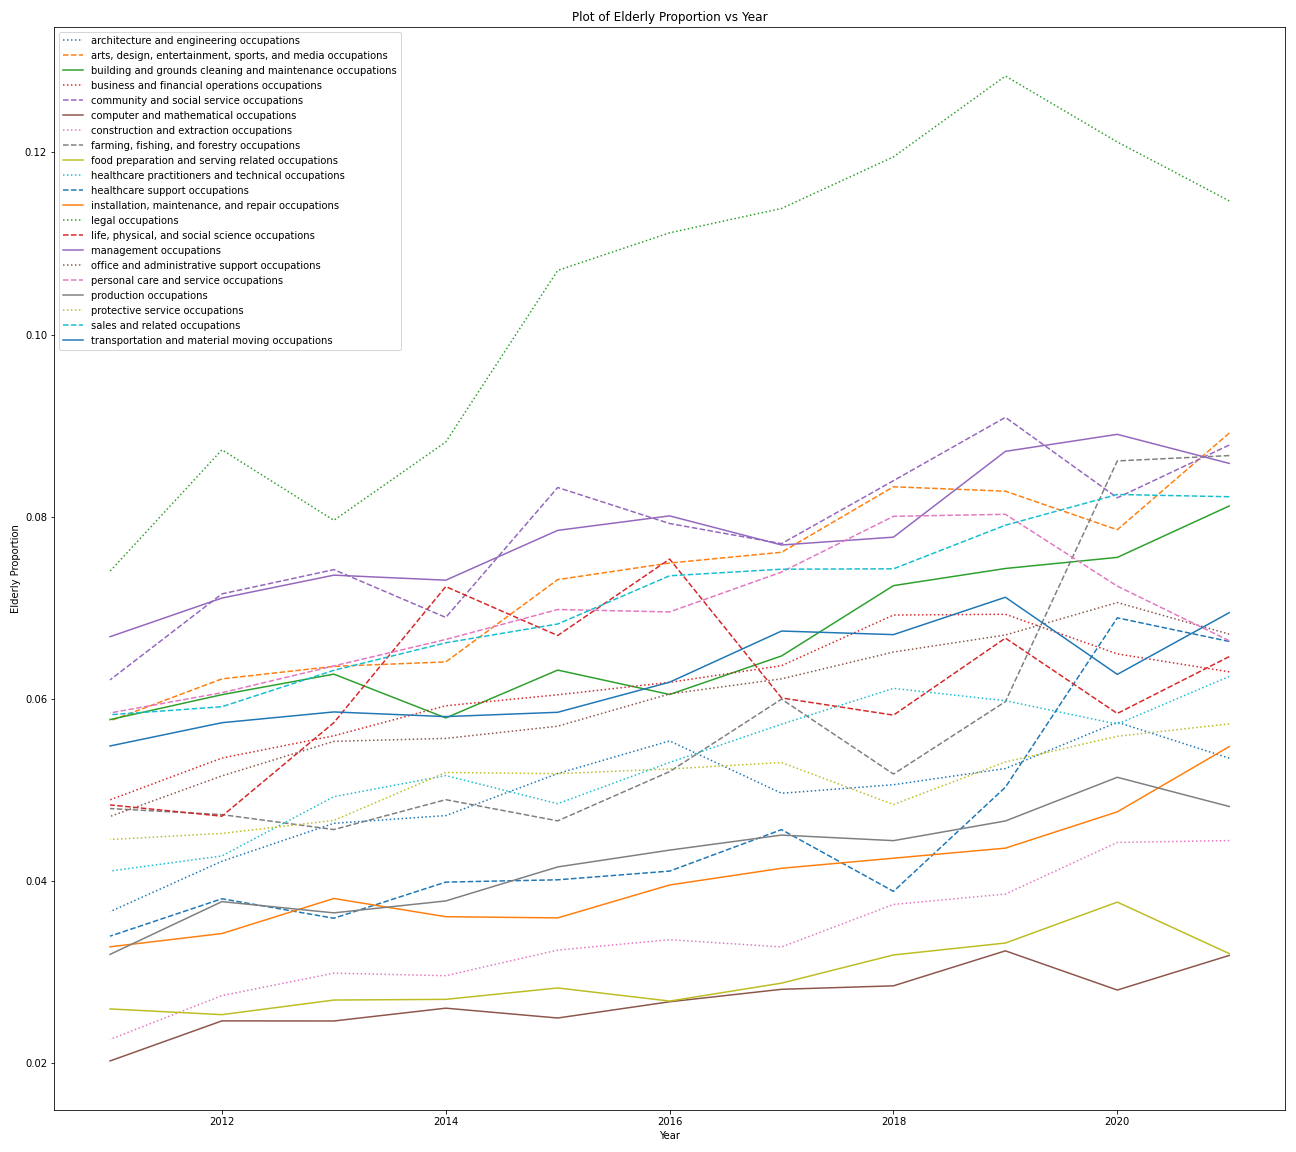
\includegraphics[width=13cm]{/Users/terencetan/Documents/Uni stuff/Engineering Science/4YP/4YP-The-Future-of-Work/Report/Figures/Elderly Proportion against Year}\label{fig:EP against year}}
	\hfill
	\subfloat[Old Proportion]{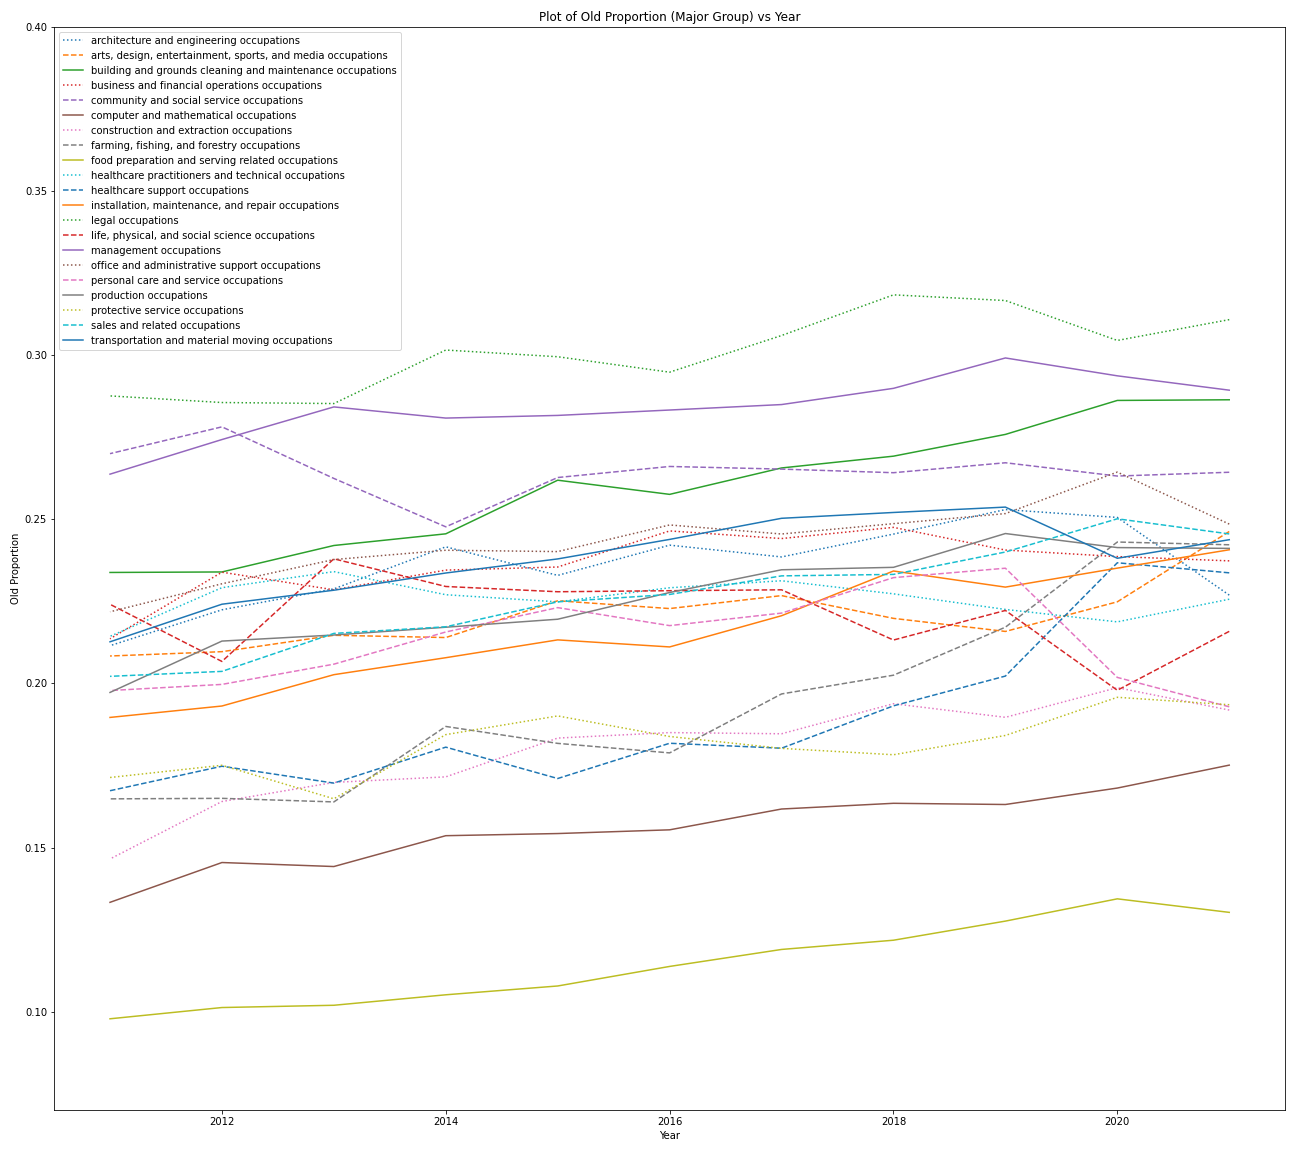
\includegraphics[width=13cm]{/Users/terencetan/Documents/Uni stuff/Engineering Science/4YP/4YP-The-Future-of-Work/Report/Figures/Old Proportion against Year}\label{fig:OP against year}}
	\hfill
	\caption{Plot of EP/OP (for each Major Groups) against Year. There is a general increase across most of the Major Group occupations, which is expected given the ageing population in the United States.}
	\label{fig:EP/OP against year}
\end{figure}

That being said, it is rather tricky to make sense of Figure \ref{fig:EP/OP against year} given that there are 21 individual plots within each of the two figures. Hence, we can calculate the relative change in EP/OP each Major Group occupation from 2011 to 2021 to obtain Figure \ref{fig:relativechange}. The `construction and extraction occupations' has the highest relative increase while the `personal care and service occupations' features the least.


\begin{figure}[!htb]
	\centering
	\subfloat[Elderly Proportion]{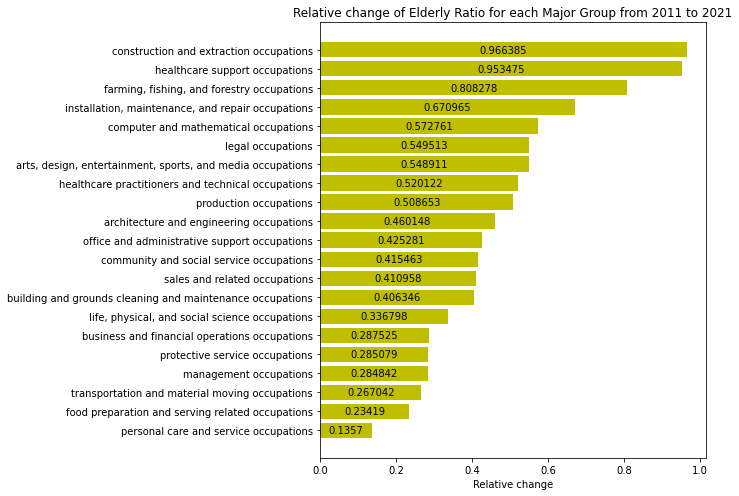
\includegraphics[width=13cm]{/Users/terencetan/Documents/Uni stuff/Engineering Science/4YP/4YP-The-Future-of-Work/Report/Figures/Relative change.png}\label{fig:Relative change of EP}}
	\hfill
	\subfloat[Old Proportion]{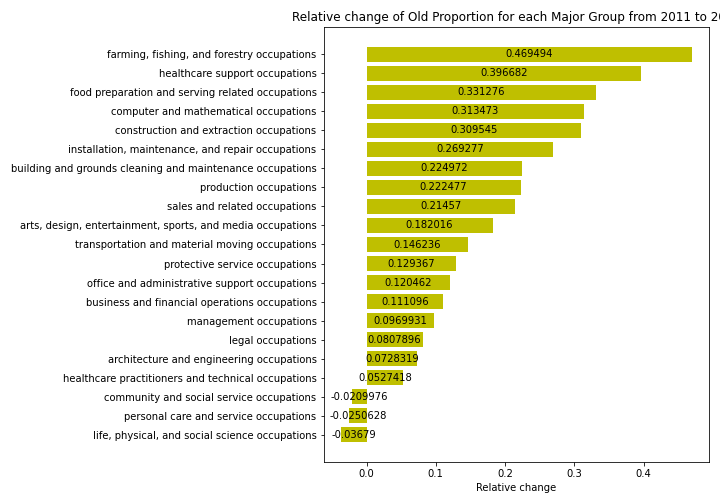
\includegraphics[width=13cm]{/Users/terencetan/Documents/Uni stuff/Engineering Science/4YP/4YP-The-Future-of-Work/Report/Figures/Relative change of OP}\label{fig:Relative change of OP}}
	\hfill
	\caption{Relative change of EP/OP for each Major Group from 2011 to 2021. This shows us which occupations experienced the most and least rapid ageing during the time period of 2011 to 2021.}
	\label{fig:relativechange}
\end{figure}


% \begin{figure}[!htb]
% 	\centering
% 	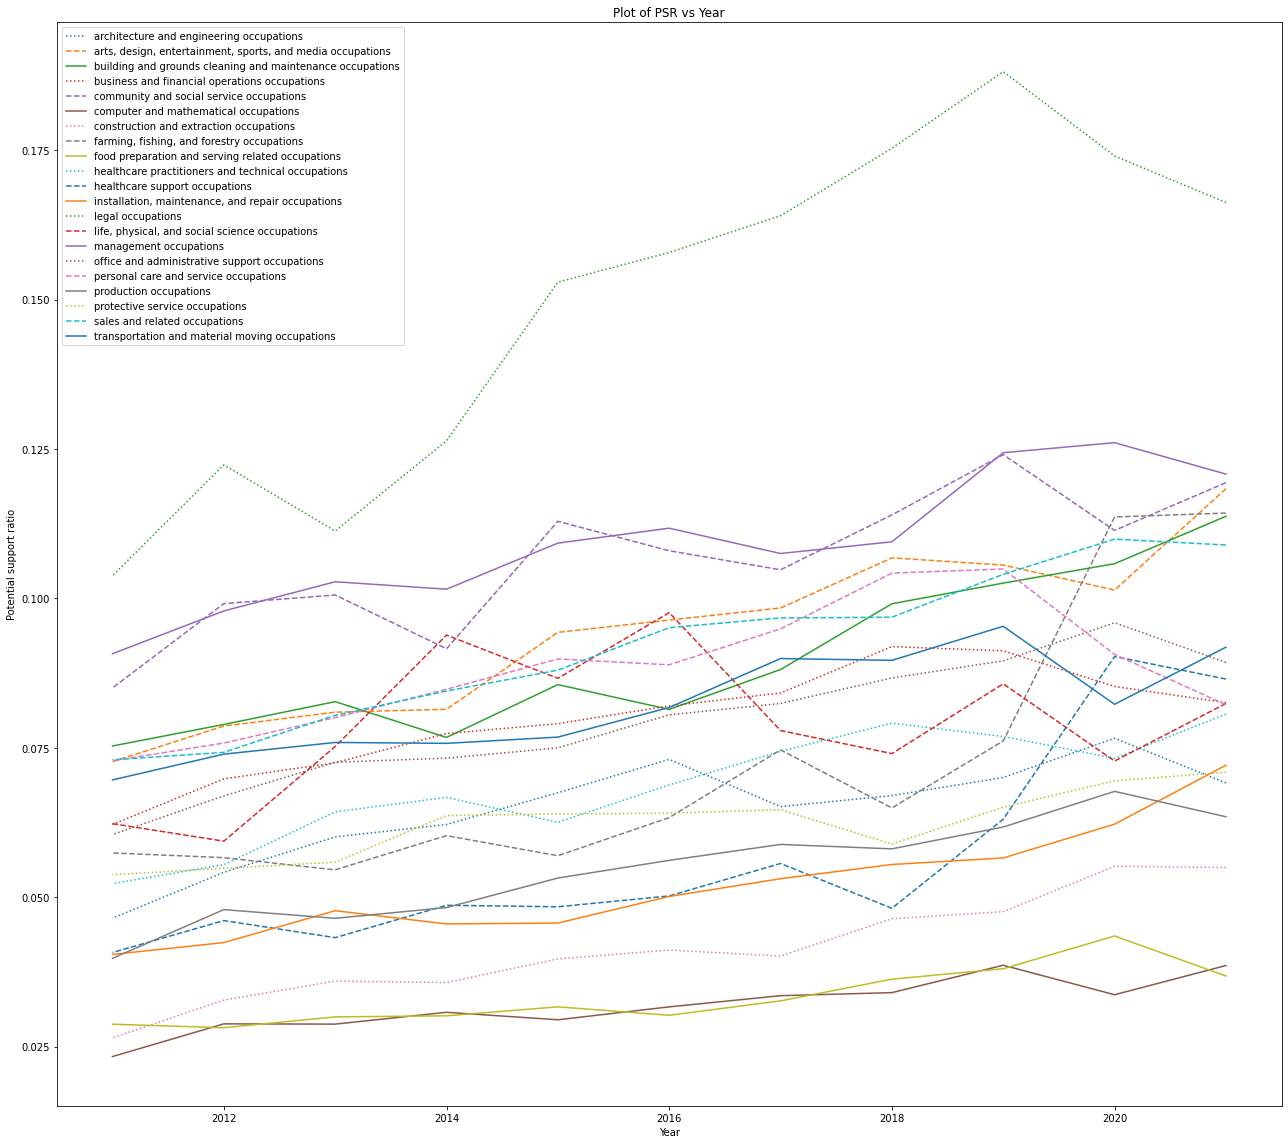
\includegraphics[width=17cm]{/Users/terencetan/Documents/Uni stuff/Engineering Science/4YP/4YP-The-Future-of-Work/Report/Figures/PSR vs Year.png}
% 	\caption{Plot of PSR vs Year for Major Groups}
% 	\label{fig:psrvsyear}
% \end{figure}

\newpage

\section{Data Analysis}

Now that we have our processed BLS dataset (with the calculated OP and EP), we can use \emph{Pandas.merge} to join it with the automatability dataset (which includes the Probability of Computerisation) from \cite{futureofemployment} based on the Detailed Occupation. This gives us a joint data set that we will refer to as \emph{joint\_auto}. Unfortunately, the BLS dataset does not feature a full list of all the Detailed Occupations, so we end up with a reduced set of Detailed Occupations in the \emph{joint\_auto} dataset. As can be seen in Figure \ref{fig:jointautoratio}, \emph{joint\_auto} only represents about 40\% of the total US civilian labour force, which is still a significant amount. However, there is the question of whether \emph{joint\_auto} is a representative sample of the population, i.e. the US civilian labour force. We shall analyse this question by treating it as a population sampling problem.

\begin{figure}[!htb]
	\centering
	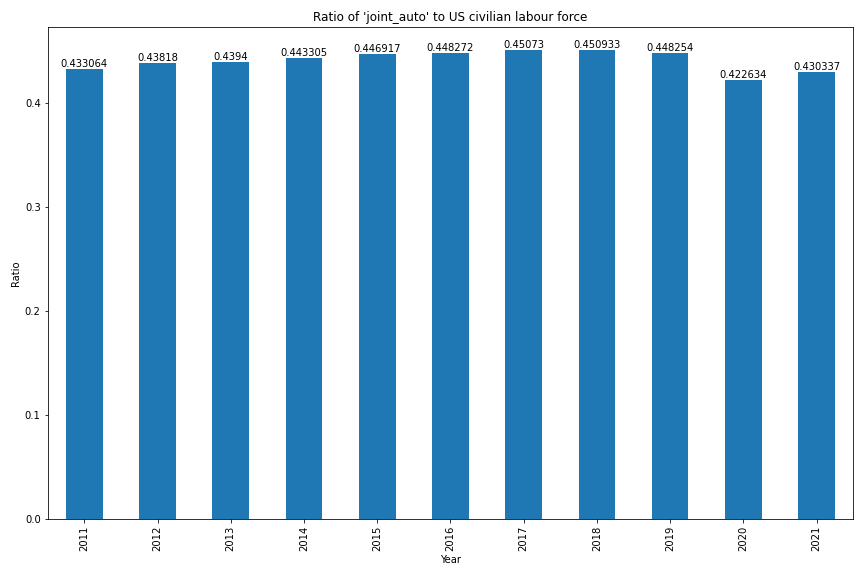
\includegraphics[width=12cm]{/Users/terencetan/Documents/Uni stuff/Engineering Science/4YP/4YP-The-Future-of-Work/Report/Figures/joint_auto ratio.png}
	\caption{Plot of ratio of \emph{joint\_auto} to US civilian labour force against Year. We can see that our \emph(joint\_auto) dataset represents a significant proportion of the total labour force, but not enough for us to generalise any trends we may find in our dataset. We will have to investigate how well our dataset represents the actual US civilian labour force.}
	\label{fig:jointautoratio}
\end{figure}


\subsection{Checking biasness}
\label{subsec:Checking biasness}
As mentioned earlier, we shall treat \emph{joint\_auto} as the sample and the US civilian labour force as the population. We shall use the Major Group occupations from our processed BLS dataset to represent the US civilian labour force since we have established its high representation in Chapter \ref{sec:prelim findings}.

We start off with a simple mean and variance comparison.  We find the mean and variance of the OP, EP, and PCom values for both the sample and population, which are shown in Table \ref{tab:mean and variance}. We can see that the means and variances match quite well for the PCom variable. For OP and EP, the means match quite closely, but the variances are off by an order of magnitude; the sample have a higher variance than the population for both OP and EP. This means that the sample have more spread-out values for OP and EP, so we must exercise caution when generalising any findings from the sample to the population. Otherwise, the sample seems fairly representative of the population. That being said, the mean and variance analysis is too simplistic to give us any concrete conclusions. Hence, we need a more sophisticated measure of the sample's representativeness of the population.

\begin{table}[]
	\centering
	\begin{tabular}{l|ll|ll}
					  & \multicolumn{2}{l|}{\textbf{Population}} & \multicolumn{2}{l}{\textbf{Sample}} \\ \cline{2-5} 
	\textbf{Variable} & Mean               & Variance            & Mean            & Variance          \\ \hline
	EP                & 0.0578             & 0.000394            & 0.0516          & 0.00334           \\ \hline
	OP                & 0.220              & 0.00190             & 0.223           & 0.0122            \\ \hline
	PCom              & 0.536              & 0.136               & 0.508           & 0.143            
	\end{tabular}
	\caption{Population/Sample mean and variance. We can see that the means and variances are very similar between the sample and the population. However, we note that the EP/OP values for the sample have higher variances compared to that of the population.}
	\label{tab:mean and variance}
\end{table}


We can look at the proportion of the total number of people employed within each Major Group with respect to the total US civilian labour force for each year. For example, Management Occupations represent 13.2\% of the US civilian labour force in 2021, 13.4\% in 2020 and so on. Transportation and Material Moving Occupations represent 6.34\% in 2011, 6.38\% in 2012 and so on. We put all of this information into one vector, which would represent the population proportion. We then map all the occupations (which are Detailed Occupations) in \emph{joint\_auto} back to their respective Major Groups, and sum up the number of people employed in each of those Detailed Occupations within the Major Groups for each year. These numbers are then divided by the total number of people employed in \emph{joint\_auto} for each year. This would tell us the proportion of each of the 21 Major Groups within \emph{joint\_auto} for each year; this sample proportion information would be placed in another vector. We want to see how well the sample proportion vector matches the population proportion vector, so we subtract the former from the latter and plot the result in Figure \ref{fig:relativeweightage}. We can see that the values along the y-axis are all fairly small. Hence, the sample has a similar makeup to the population in terms of the relative weightage of each of the Major Groups.

Given our above biasness tests, we can make the reasonable assumption that our sample is fairly representative of the population, and any findings obtained from the sample can be generalised to the population to a certain extent.


\begin{figure}[!htb]
	\centering
	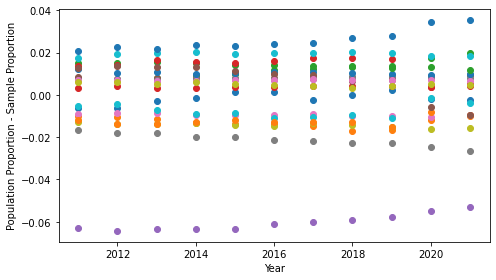
\includegraphics[width=12cm]{/Users/terencetan/Documents/Uni stuff/Engineering Science/4YP/4YP-The-Future-of-Work/Report/Figures/sample test.png}
	\caption{Plot of the difference between the population proportion and the sample proportion against Year. The low values along the y-axis shows that the relative weightage of each of the Major Groups within the sample is similar to that of the population. Hence, the sample has a similar makeup to the population in terms of the Major Groups.}
	\label{fig:relativeweightage}
\end{figure}

\subsection{Exploration of Data}
Now that we have established the representativeness of the sample, we can go about exploring the dataset. The first thing we do is to create a scatterplot of the Detailed Occupations within \emph{joint\_auto}, with the EP/OP values on the y-axis and the PCom values on the x-axis. We also scale each data point relative to the total number of people employed within that occupation, i.e. occupations with more people will be bigger on the plot. This gives us Figure \ref{fig:EP/OP against PCom}, which we can see has no obvious trends. Zooming in on specific regions of the scatterplot (e.g. the region of high PCom) also yields no significant patterns. We do note that the majority of employed workers are concentrated in either the low PCom region or the high PCom region, with relatively few in between. This is consistent with the findings from \cite{osborne2017future}, and is another piece of evidence that our assumption that \emph{joint\_auto} is fairly representative of the US civilian labour force is reasonable as discussed in Chapter \ref{subsec:Checking biasness}. 

Our next step of exploration is to take the base 10 logarithmic of EP/OP and PCom, and plot the former against the latter in a scatterplot, as shown in Figure \ref{fig:logEP/OP against PCom}. Interestingly, the $\log_{10}$(OP) plot in Figure \ref{fig:logOP against PCom} seems to show a slight downward trend as $\log_{10}$(PCom) increases; plotting the scatterplot on a logarithmic scale seems to have revealed a previously hard-to-spot trend. This trend suggests that 'older' occupations tend to be less likely to be computerised. This makes intuitive sense for occupations such as management; \cite{osborne2017future} notes that management occupations tend to be at low risk of computerisation due to the high degree of social intelligence required for them, and people in management positions would also tend to be older since such occupations (especially the ones like Chief Executive Officer) would be biased towards those with more work experience. There is also some evidence that high skilled workers, who would generally be less likely to have their jobs computerised, tend to retire later than low skilled workers (\cite{HimmelreicherRalfK.2009Saao}).

% \begin{table}[]
% 	\centering
% 	\begin{tabular}{l|ll|ll}
% 					  & \multicolumn{2}{l|}{\textbf{Population}} & \multicolumn{2}{l}{\textbf{Sample}} \\ \cline{2-5} 
% 	\textbf{Variable} & Mean               & Variance            & Mean            & Variance          \\ \hline
% 	EP                & 0.0578             & 0.000394            & 0.0516          & 0.00334           \\ \hline
% 	OP                & 0.220              & 0.00190             & 0.223           & 0.0122            \\ \hline
% 	PCom              & 0.536              & 0.136               & 0.508           & 0.143            
% 	\end{tabular}
% 	\caption{Population/Sample mean and variance. We can see that the means and variances are very similar between the sample and the population. However, we note that the EP/OP values for the sample have higher variances compared to that of the population.}
% 	\label{tab:mean and variance}
% \end{table}




\begin{figure}[!htb]
	\centering
	\subfloat[Elderly Proportion]{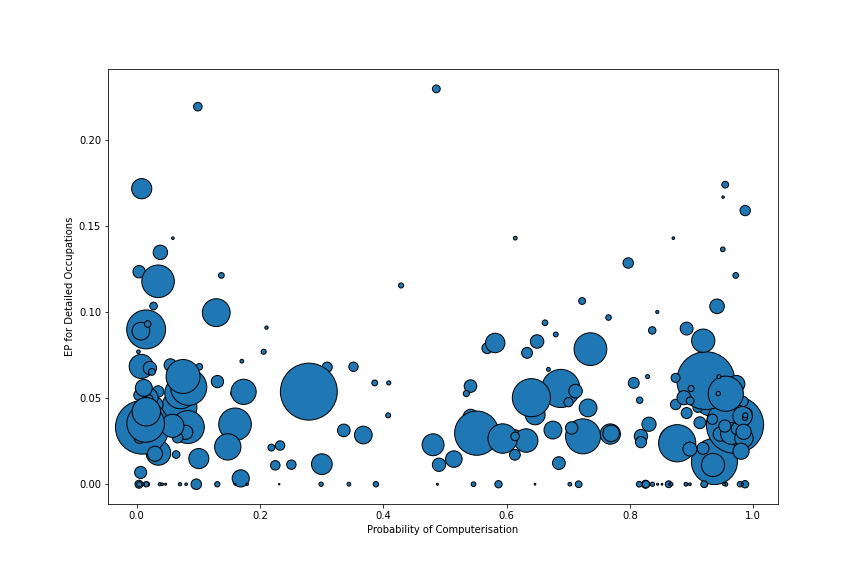
\includegraphics[width=15cm]{/Users/terencetan/Documents/Uni stuff/Engineering Science/4YP/4YP-The-Future-of-Work/Report/Figures/Scatterplot of EP for DO}\label{fig:EP against PCom}}
	\hfill
	\subfloat[Old Proportion]{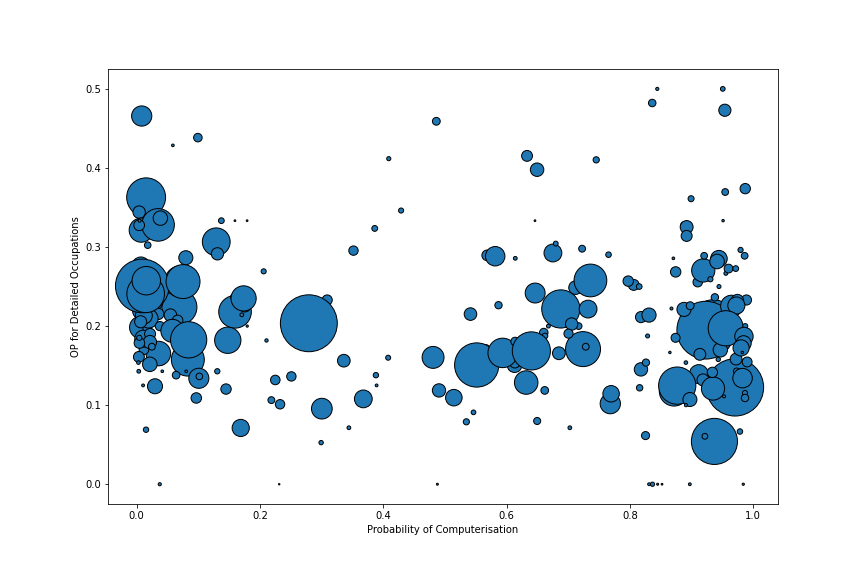
\includegraphics[width=15cm]{/Users/terencetan/Documents/Uni stuff/Engineering Science/4YP/4YP-The-Future-of-Work/Report/Figures/Scatterplot of OP for DO}\label{fig:OP against PCom}}
	\hfill
	\caption{Plot of EP/OP (for each Detailed Occupation) against PCom. There seems to be no obvious patterns or trends present.}
	\label{fig:EP/OP against PCom}
\end{figure}


\begin{figure}[!htb]
	\centering
	\subfloat[Elderly Proportion]{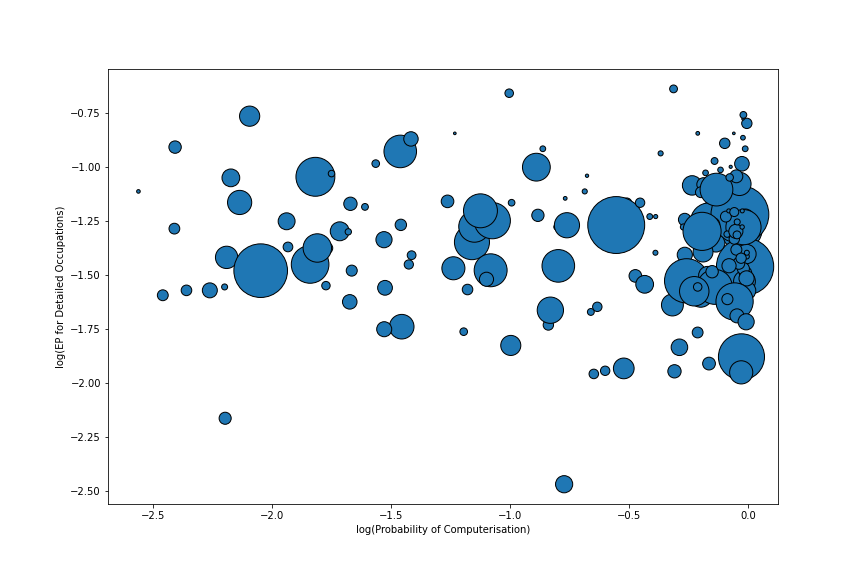
\includegraphics[width=15cm]{/Users/terencetan/Documents/Uni stuff/Engineering Science/4YP/4YP-The-Future-of-Work/Report/Figures/Scatterplot of log(EP) for DO}\label{fig:logEP against PCom}}
	\hfill
	\subfloat[Old Proportion]{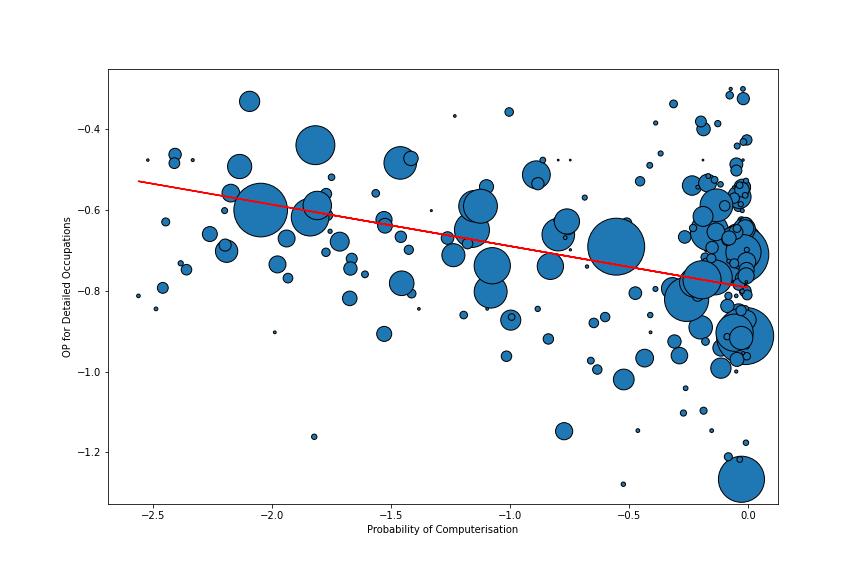
\includegraphics[width=15cm]{/Users/terencetan/Documents/Uni stuff/Engineering Science/4YP/4YP-The-Future-of-Work/Report/Figures/Scatterplot of log(OP) for DO}\label{fig:logOP against PCom}}
	\hfill
	\caption{Plot of $\log_{10}$(EP)/$\log_{10}$(OP) (for each Detailed Occupation) against $\log_{10}$(PCom). There seems to be a slight downward trend for the $\log_{10}$(OP) plot. This suggests that occupations that are less susceptible to computerisation tend to have a higher proportion of old people.}
	\label{fig:logEP/OP against PCom}
\end{figure}



\subsection{Linear Regression}

\subsection{Probably Approximately Correct (PAC) Learning}
Suppose we have an unknown target set \emph{T} from which we obtained independent and identically distributed (i.i.d.) samples $\delta_{1},...,\delta_{m}$. Using the \emph{m} samples, we want to construct a hypothesis set $H_{m}$ that approximates \emph{T}. The framework we use to learn $H_{m}$ is known as PAC Learning.

Of course, we want $H_{m}$ to approximate \emph{T} as close as possible, such that the probability of a new sample $\delta$ from \emph{T} not belonging in $H_{m}$ is less than or equal to an arbitrary threshold probability $\epsilon$, i.e. $\mathbb{P}(\delta \in \emph{T} \setminus H_{m}) \leq \epsilon$. Since $H_{m}$ depends on the i.d.d. random samples $\{\delta_{1},...,\delta_{m}\}$, it is also random. This means that $\mathbb{P}(\delta \in \emph{T} \setminus H_{m}) \leq \epsilon$ is itself a random variable, allowing us to quantify a confidence for it:
\begin{equation}
	\label{eq:1}
	\mathbb{P}^{m} \{\delta_{1},...,\delta_{m}: \mathbb{P}(\delta \in \emph{T} \setminus H_{m}) \leq \epsilon \} \geq 1 - q(m,\epsilon),
\end{equation}
where $1 - q(m,\epsilon)$ is a lower bound to our confidence that the probability of a new sample not belong in $H_{m}$ is less than or equal to $\epsilon$. We refer the reader to (\cite{paclearning1}) for a more comprehensive introduction to this concept.

Furthermore, consider the following scenario program:
\begin{equation}
	\label{eq:2}
	\begin{array}{rrclcl}
	\displaystyle \min_{x \in \mathbb{R}^{n_{x}}} & \multicolumn{3}{l}{c^{T}x}\\
	\textrm{s.t.} & g(x,\delta_{i}) \leq 0, \text{for all i = 1,...,m}\\
	\end{array}
	\end{equation}
Suppose $\delta_{i}$ belongs to an uncertainty space $\Delta$, i.e. $\delta_{i} \in \Delta$ for $i = 1,...,m$, and we have obtained the optimal solution $x^{*}_{m}$ to the scenario program in Equation \ref{eq:2}. If we then want to find out if a new $\delta\in \Delta$ will violate the constraint $g(x^{*},\delta) \leq 0$, we can use Equation \ref{eq:1} to quantify the probability of such a constraint violation happening. Let $T=\Delta$, $H_{m} = (\delta \in \Delta: g(x^{*}_{m},\delta) \leq 0)$, i.e. the set of samples for which $x^{*}_{m}$ remains feasible, and we get the following:

\begin{equation}
	\label{eq:3}
	\mathbb{P}^{m} \{\delta_{1},...,\delta_{m}: \mathbb{P}(\delta \in \Delta: g(x^{*}_{m},\delta) > 0) \leq \epsilon \} \geq 1 - q(m,\epsilon),
\end{equation}
where $\mathbb{P}(\delta \in \Delta: g(x^{*}_{m},\delta) > 0)$ is the probability that a new sample $\delta\in \Delta$ violates the constraint $(g(x^{*}_{m},\delta) \leq 0)$. Similar to Equation \ref{eq:1}, the probability of such a constraint violation should ideally to less than or equal to an arbitrary value $\epsilon$, and our confidence of that happening is at least $1 - q(m,\epsilon)$.

\newpage
\printbibliography[heading=bibintoc]


\end{document}
